\section{Architecture for Video Streaming Provisioning}
"\label{sec:system-archi}

{\color{blue} This section explains the architecture system, and what it is  for, explaining some protocols flowcharts. Studying the protocols and focusing in the system part of the experiments.}

This section explains the main contribution of the paper. We first provide an overview of the proposed video streaming service architecture using Controller-assisted and SVC including its rationale. The remaining subsections describe the implementation of this service architecture.

\subsubsection{Impact of Fog Multi-tier Networks}

In Figure~\ref{fig:impact-two-layers}, we present two approaches to address the impact identified for requesting the multimedia content in different layers on the network. The charts show the results of bit rate, interruptions, buffer and representations switch, respectively from left to right over the simulation time. As we can see, both users have had no interruptions throughout the video, besides the initial interruption until the start of the video. However, the user who received the video on the nearest fog layer had a higher bit rate than the other user. As well as the buffer was soon filled and the user had the best possible resolution of the video. Whereas the user who received the video from a more distant layer, in some moments, worked with the buffer at the limit and had to constantly switch resolutions so that there is no interruption during the video execution.

\subsection{Resource Requirements based on QoS}

Manage the QoE users refer to those service where the satisfaction guarantees can be centrally controlled by the controller. The Controller can address this problem by creating a control channel to managed-quality video streaming services over the edge-cloud network.

\subsection{Application-to-network mapping}


\subsection{QoE Metrics}

To quantify the users' QoE, we will describe the QoE metrics used to calculate the user satisfaction. 

\subsubsection{Chunk Quality ($q(r_i)$)} Each video has $N$ chunks and is encoded with $L$ bitrate levels. $r_i$ represents a specific bitrate level. At each step $i$, the quality of chunk $i$ which is encoded at $l_i$ is defined as:

$$
q(r_i) = a_1 * log(a_2 * (r_i/ r_{|L|}))
$$


\subsubsection{Average Video Quality($Q_{avg}$):} To know the average of the video quality of each user during the video streaming, we calculate as:

$$
Q_{avg} = \sum_{i \in N} q(r_i)
$$

\subsubsection{Number of Stalls}

\subsubsection{Video Quality Switches}

To quantify the QoE we define a function with the above metrics:

$$
QoE_i = \alpha_1 + \alpha_2 + \alpha_3 + \alpha_4
$$

Where the values 1 = bad, 2 = poor, 3 = fair, 4 = good, and 5 = excellent.

\begin{figure}
    \centering
    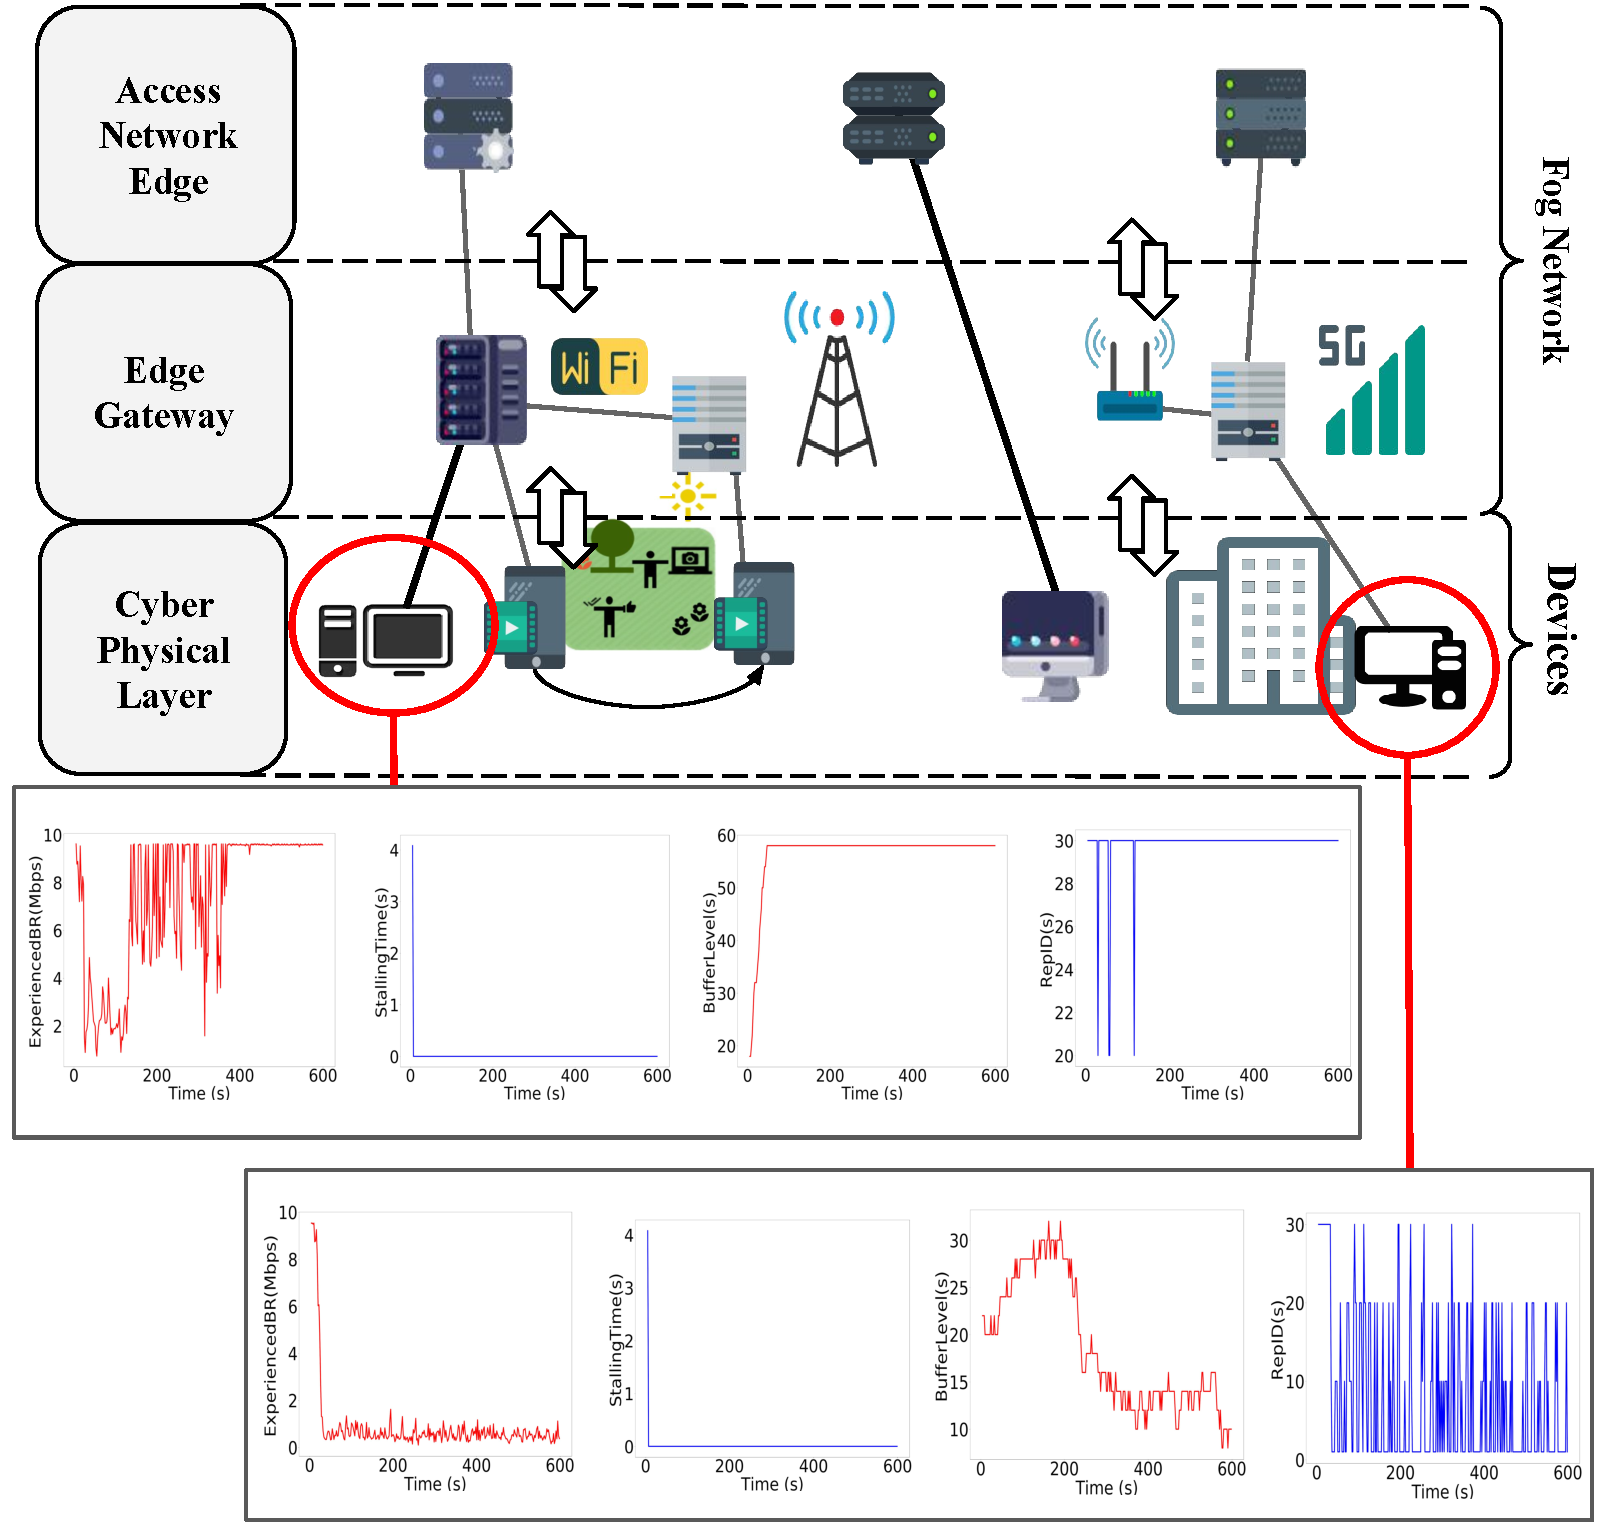
\includegraphics[width=0.9\linewidth]{images/qoe-multi-level.pdf}
    \caption{Overview of the multi-tier-based  network environmental simulation.}
    \label{fig:impact-two-layers}
\end{figure}
